
\section{Создание экспериментального образца}
//фотография
//характеристики
//процесс сборки
//проверка работы
//перенести подробности из парт2
\subsection{Выбор компонентов квадрокоптера}
Проведен анализ рынка радиоуправляемых квадрокоптеров и замечено, что готовых вариантов, подходящих для взаимодействия с разрабатываемой наземной станцией, нет. В связи с чем необходимо подобрать компоненты и собрать вручную.

\subsection{Выбор компонентов наземной станции}
\subsection{Сборка}
\subsection{Проверка работы экспериментального образца}
% ~\ref{fig:map}
\begin{figure}[H]
	\centering
	
\includegraphics[width=0.5\linewidth]{pics/map}
	\caption{Карта маркеров
	}
	\label{fig:map}
\end{figure}

% ~\ref{fig:aruco_detect}
\begin{figure}[H]
	\centering
	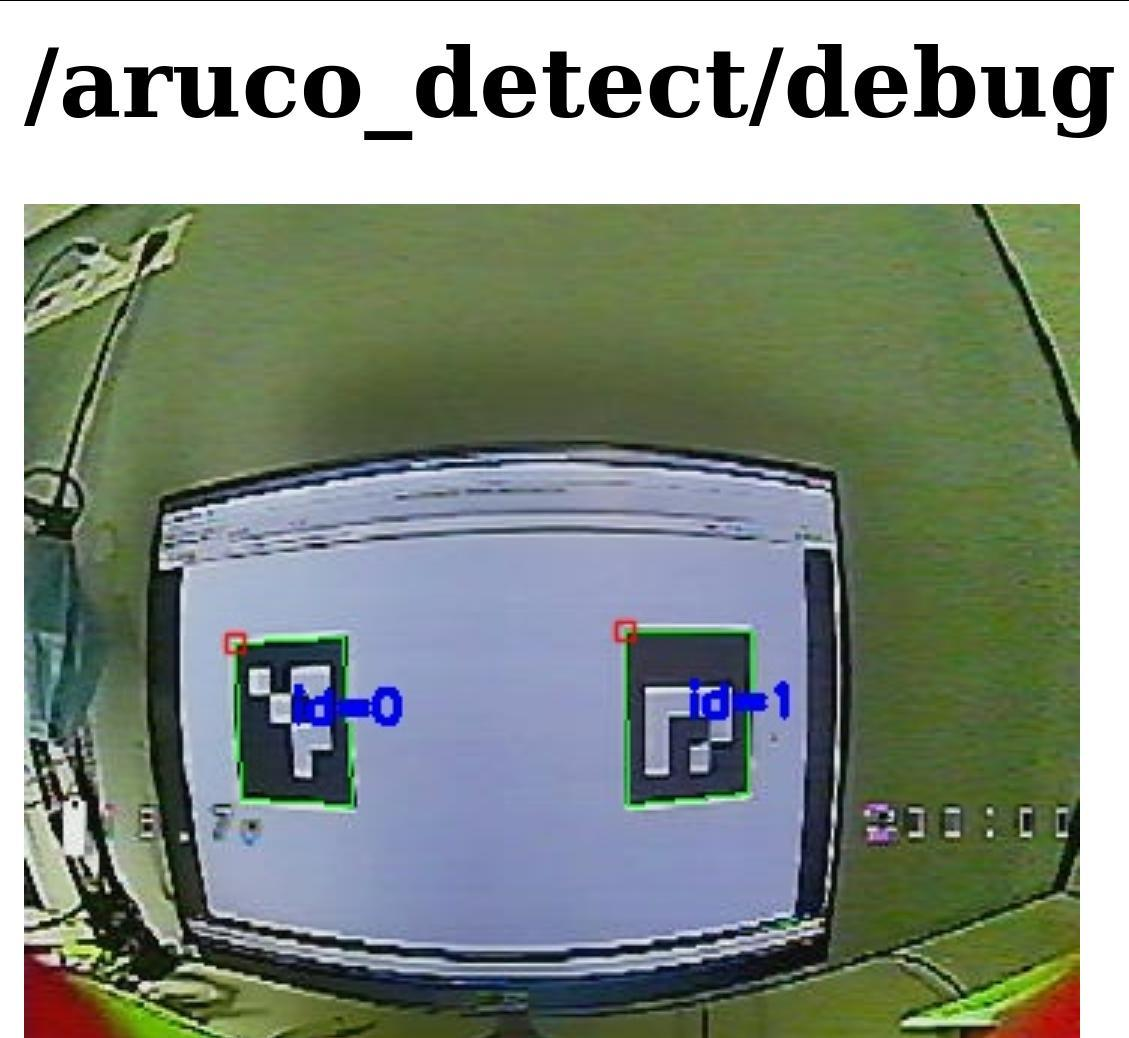
\includegraphics[width=0.5\linewidth]{pics/aruco_detect}
	\caption{Инициализация aruco маркеров
	}
	\label{fig:aruco_detect}
\end{figure}

% ~\ref{fig:time}
\begin{figure}[H]
	\centering
	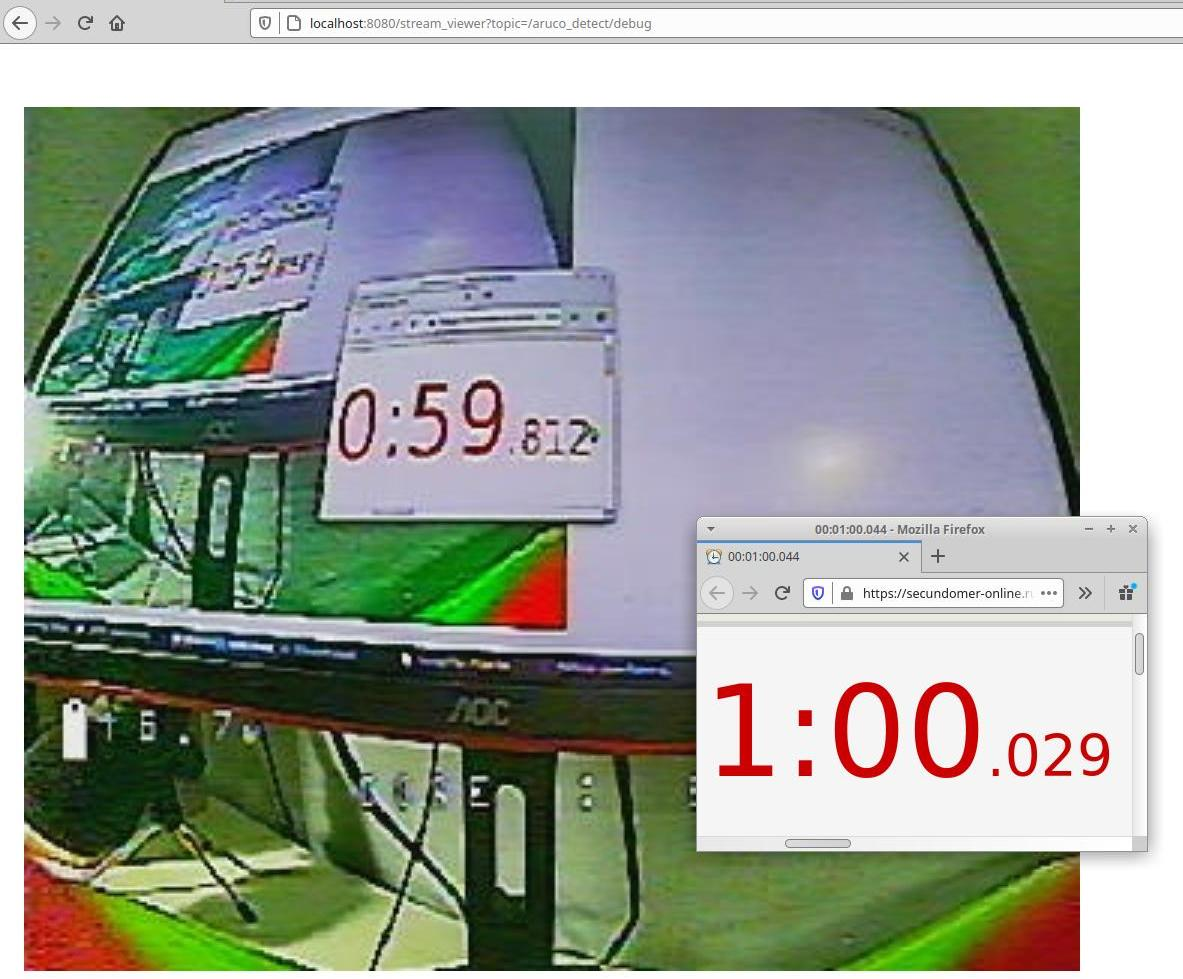
\includegraphics[width=0.5\linewidth]{pics/time}
	\caption{Время задержки% 0.2с
	}
	\label{fig:time}
\end{figure}
\subsection{smthng}
